\begin{frame}[fragile]{Tutorial: Two-site states}

\begin{columns}

\begin{column}{5cm}

\begin{onlyenv}<1->
\begin{lstlisting}[language=JuliaLocal, style=julia, mathescape, basicstyle=\scriptsize\ttfamily]
$\psi$ = ITensor(i1, i2)
$\psi$[i1=>1, i2=>2] = 1/√2
$\psi$[i1=>2, i2=>1] = 1/√2

$\psi$ = (Zp1 * Zm2 +
     Zm1 * Zp2)/√2
\end{lstlisting}
\end{onlyenv}

\begin{onlyenv}<3->
\begin{lstlisting}[language=JuliaLocal, style=julia, mathescape, basicstyle=\scriptsize\ttfamily]
inner(ZpZm, $\psi$) == 1/√2


U, S, V = svd(ZpZm, i1);
diag(S) == [1, 0]

U, S, V = svd($\psi$, i1);
diag(S) == [1/√2, 1/√2]
\end{lstlisting}
\end{onlyenv}

\end{column}

\begin{column}{5cm}

\begin{onlyenv}<1-1>
(|Z+$\rangle$|Z-$\rangle$ + |Z-$\rangle$|Z+$\rangle$)/√2 \\
~\\
~\\
~\\
From single-site states \\
\end{onlyenv}

\begin{onlyenv}<2->
\vspace*{0.0cm}
\begin{center}
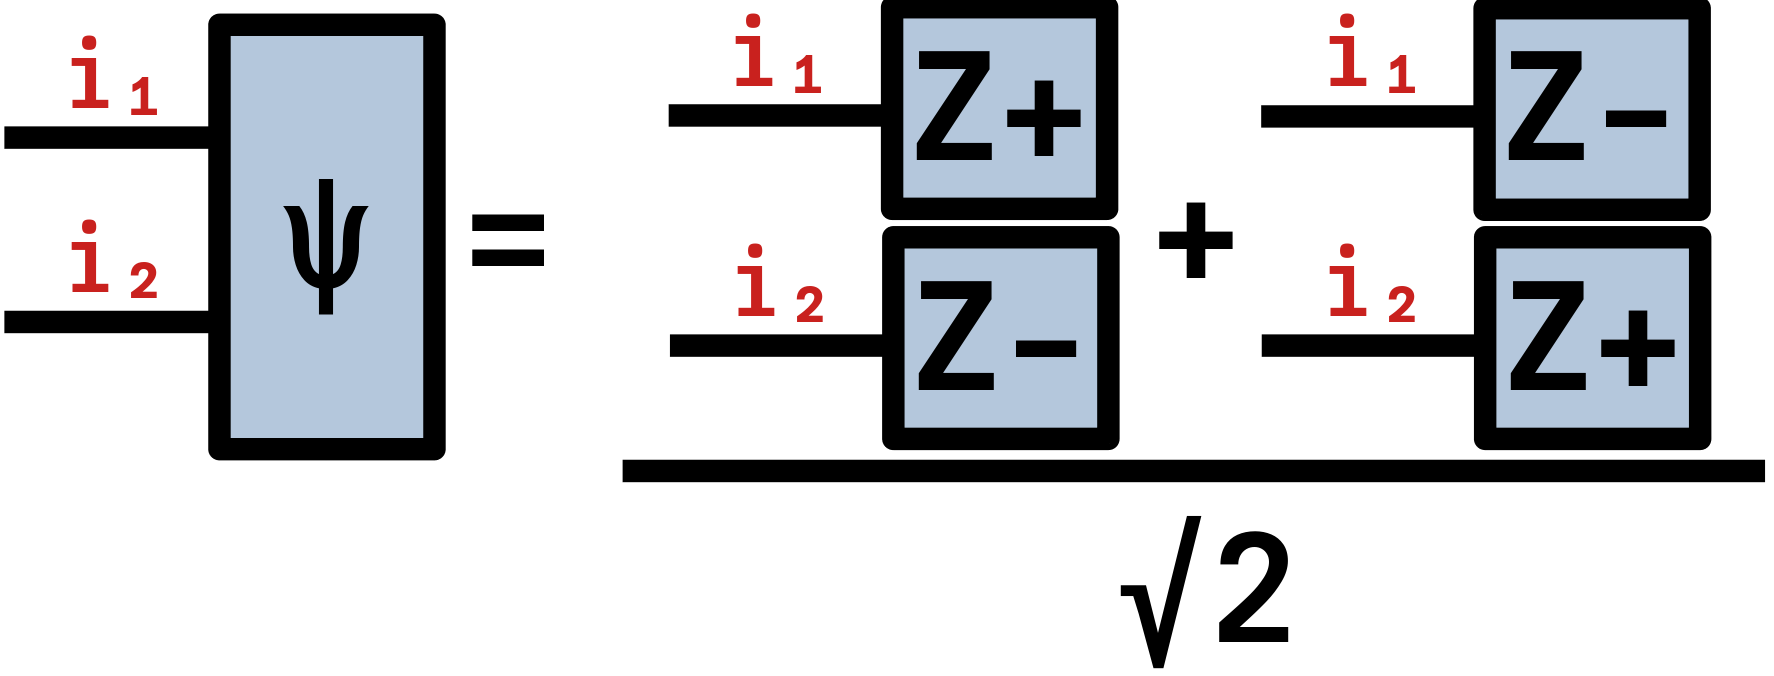
\includegraphics[width=1.0\textwidth]{
  slides/assets/cat12.png
}
\end{center}
\vspace*{0.0cm}
\end{onlyenv}

%% \begin{onlyenv}<3-3>
%% ~\\
%% $\approx$ 1 \\
%% $\approx$ 1/√2 \\
%% ~\\
%% ~\\
%% $\approx$ [1, 0] \\
%% ~\\
%% ~\\
%% $\approx$ [1/√2, 1/√2]
%% \end{onlyenv}

\begin{onlyenv}<3->
\vspace*{0.0cm}
\begin{center}
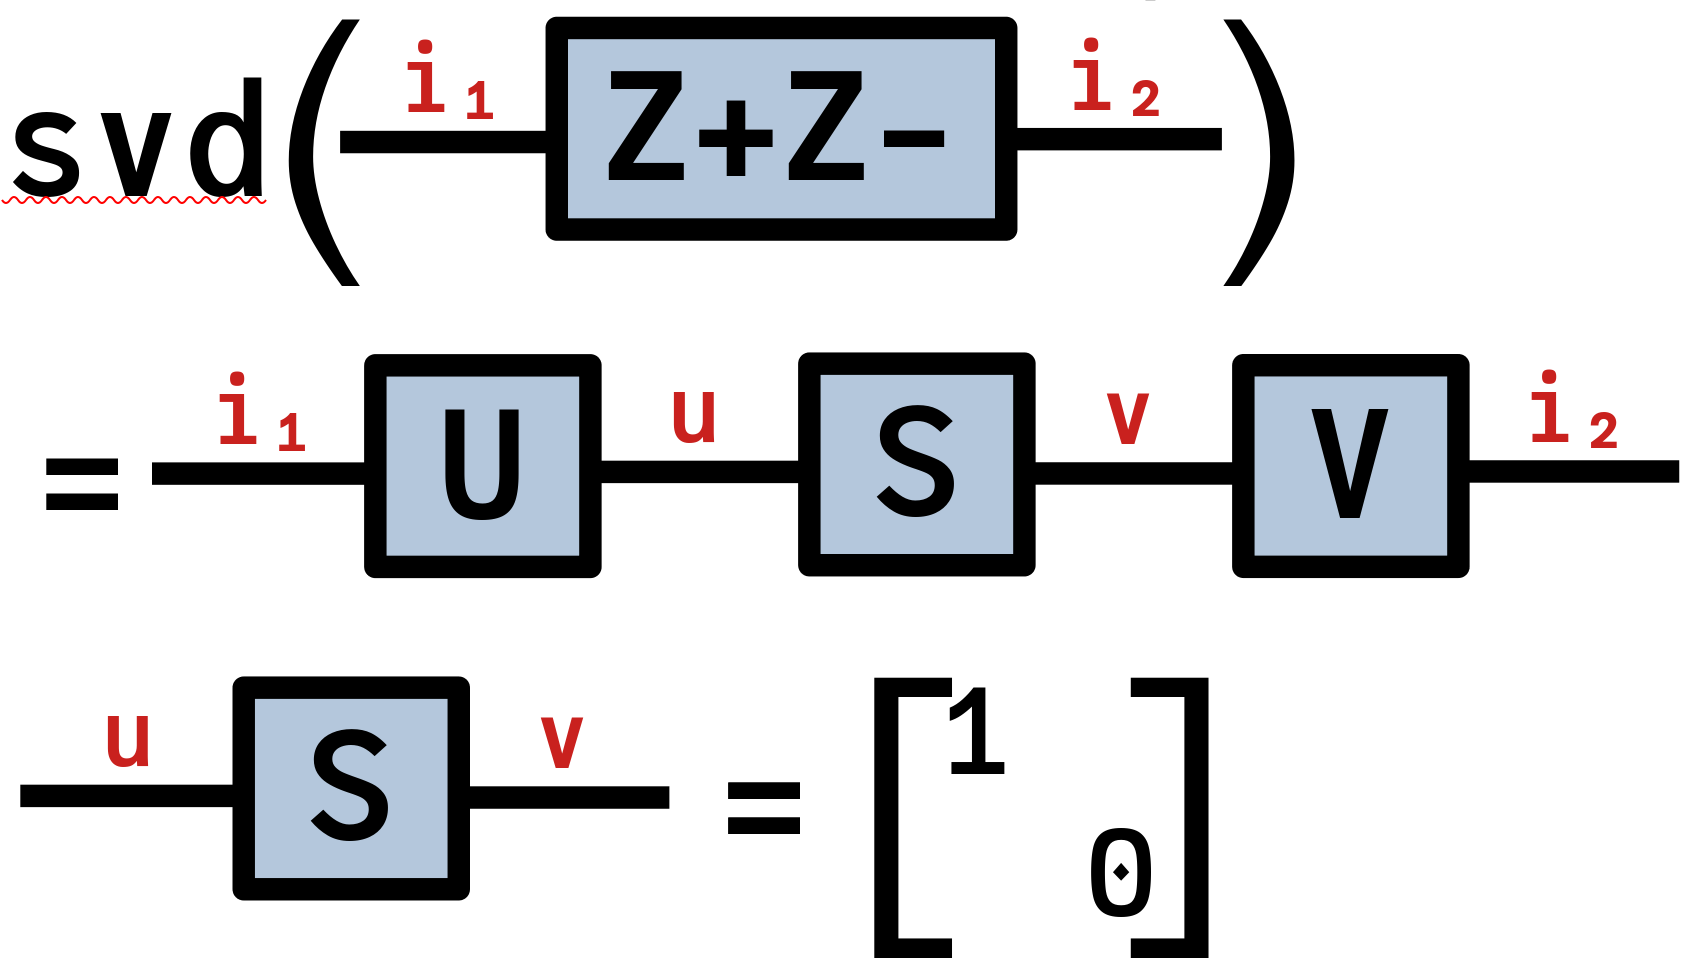
\includegraphics[width=0.7\textwidth]{
  slides/assets/svd_ZpZm12.png
}
\end{center}
\end{onlyenv}

\begin{onlyenv}<4->
\begin{center}
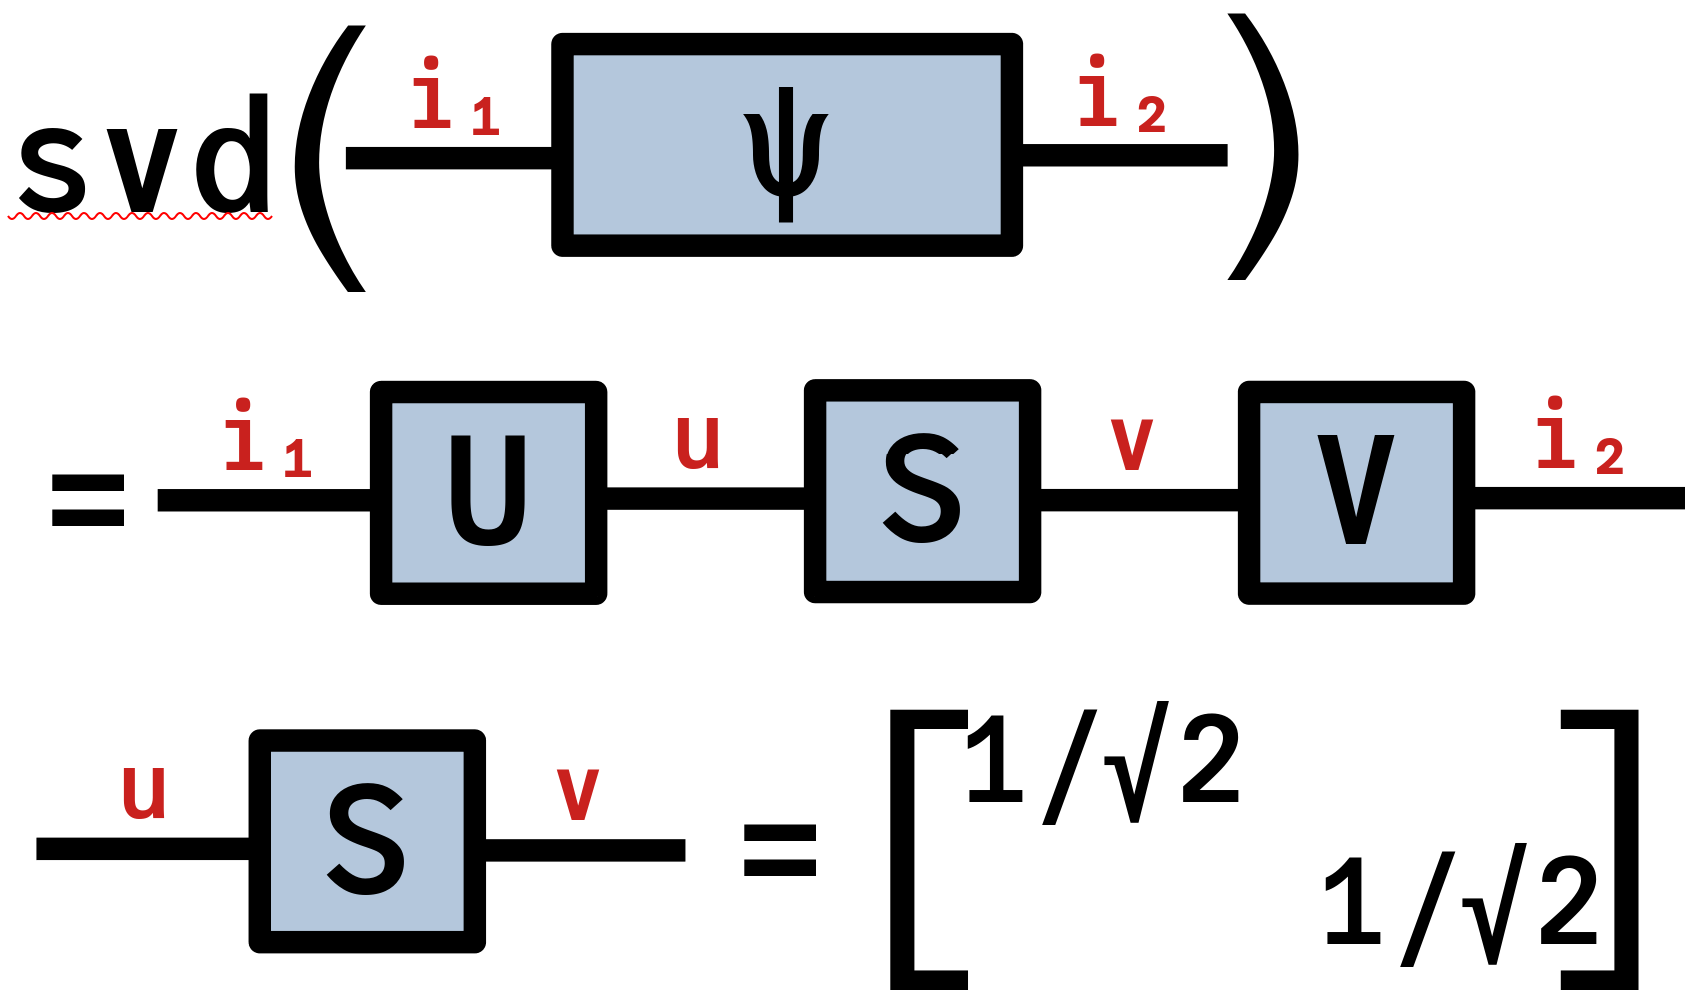
\includegraphics[width=0.7\textwidth]{
  slides/assets/svd_cat12.png
}
\end{center}
\vspace*{0.0cm}
\end{onlyenv}

\end{column}

\end{columns}

\end{frame}
